\section{Auswertung}
\noindent Im folgenden Kapitel werden die gemessenen Werte und die benötigten Umrechnungen tabellarisch dargestellt,
Ausgleichskurven für die Verläufe von $T_1$ und $T_2$, sowie deren Differentialkoeffizienten berechnet. Darauf 
folgt die berechnung der realen Güteziffer $v$, des Massendurchsatzes $\frac{\increment m}{\increment t}$, und der 
Kompressorleistung. 

\subsection{Messwerte}
\noindent In der Folgenden Tabelle sind die Messwerte Zeit $t$ in Minuten und Sekunden, die Temperaturen 
$T_1$ und $T_2$ jeweils in grad Celsius und Kelvin, sowie die Drücke $p_1$ und $p_2$ in Bar und die 
Kompressorleistung $N$ in Watt aufgeführt.
\begin{table}
  \centering
  \label{Datensatz}
  \caption{Daten und deren Umrechnung}
  \sisetup{table-format=1.2}
  \begin{tabular}{S[table-format=3.2] S S S S S S S S [table-format=3.2]}
    \toprule
    {$t$[min]} & {$t$[s]}& {$T_1$[°C]} & {$T_1$[K] } &{$p_1$[Bar]}& {$T_2$[°C]} & {$T_2$[K]} & {$p_2$[Bar]} & {$N$[W]}\\
    \midrule   
0  &     0 & 21.7 & 294.85 & 4.0  &	  21.7  & 294.85 & 4.1 &  120\\
1  &	  60 & 23.0 &	296.15 & 5.0  &	  21.7	& 294.85 & 3.2 &  120\\
2  &	 120 & 24.3 &	297.45 & 5.5  & 	21.6	& 294.75 & 3.4 &	120\\
3  &	 180 & 25.3 &	298.45 & 6.0  & 	21.5	& 294.65 & 3.5 &	120\\
4  &	 240 & 26.4 &	299.55 & 6.0  & 	20.8	& 293.95 & 3.5 &	120\\
5  &	 300 & 27.5 &	300.65 & 6.0  & 	20.1	& 293.25 & 3.4 &	120\\
6  &	 360 & 28.8 &	301.95 & 6.5  & 	19.2	& 292.35 & 3.3 &	120\\
7  &	 420 & 29.7 &	302.85 & 6.5  & 	18.5	& 291.65 & 3.2 &	120\\
8  &	 480 & 30.9 &	304.95 & 7.0  & 	17.7	& 290.85 & 3.2 &	120\\
9  &	 540 & 31.9 &	305.05 & 7.0  & 	16.9	& 290.05 & 3.0 &	120\\
10 &	 600 & 32.9 &	306.05 & 7.0  & 	16.2	& 289.35 & 3.0 &	120\\
11 &	 660 & 33.9 &	307.90 & 7.5  & 	15.5	& 288.65 & 2.9 &	120\\
12 &	 720 & 34.8 &	307.95 & 7.5  & 	14.9	& 288.05 & 2.8 &	120\\
13 &	 780 & 35.7 &	308.85 & 8.0  & 	14.2	& 287.35 & 2.8 &	120\\
14 &	 840 & 36.7 &	309.85 & 8.0  & 	13.6	& 286.75 & 2.7 &	120\\
15 &	 900 & 37.6 &	310.75 & 8.0  &	  13.0	& 286.15 & 2.6 &	120\\
16 &	 960 & 38.4 &	311.55 & 8.5  & 	12.4	& 285.55 & 2.6 &	120\\
17 &	1020 & 39.2 &	312.35 & 8.5  & 	11.7	& 284.85 & 2.6 &	120\\
18 &	1080 & 40.0 &	313.15 & 9.0  & 	11.3	& 284.45 & 2.5 &	120\\
19 &	1140 & 40.7 &	313.85 & 9.0  & 	10.9	& 284.05 & 2.5 &	120\\
20 &	1200 & 41.4 &	314.55 & 9.0  & 	10.4	& 283.55 & 2.4 &	120\\
21 &	1260 & 42.2 &	315.35 & 9.0  &	   9.9	& 283.05 & 2.4 &	120\\
22 &	1320 & 42.9 &	316.05 & 9.5  & 	 9.5	& 282.65 & 2.4 &	120\\
23 &	1380 & 43.6 &	316.75 & 9.5  & 	 9.1	& 282.25 & 2.4 &	120\\
24 &	1440 & 44.3 &	317.45 & 10.0 &	   8.7	& 281.85 & 2.4 &	120\\
25 &	1500 & 44.9 &	318.05 & 10.0 &	   8.3	& 281.45 & 2.4 &	120\\
26 &	1560 & 45.5 &	318.65 & 10.0 &	   8.0	& 281.15 & 2.3 &	120\\
27 &	1620 & 46.1 &	319.25 & 10.0 &	   7.7	& 280.85 & 2.2 &	122\\
28 &	1680 & 46.7 &	319.85 & 10.5 &	   7.4	& 280.55 & 2.2 &	122\\
29 &	1740 & 47.3 &	320.45 & 10.5 &	   7.1	& 280.25 & 2.2 &	122\\
30 &	1800 & 47.8 &	320.95 & 10.75&	   6.8	& 279.95 & 2.2 &	122\\
31 &	1860 & 48.4 &	321.55 & 11.0 &	   5.6	& 278.75 & 2.2 &	122\\
32 &	1920 & 48.9 &	322.05 & 11.0 &	   4.3	& 277.45 & 2.2 &	122\\
33 &	1980 & 49.4 &	322.55 & 11.0 &	   3.4	& 276.55 & 2.2 &	122\\
34 &	2040 & 49.9 &	323.05 & 11.0 &	   3.0	& 276.15 & 2.2 &	122\\
35 &	2100 & 50.3 &	323.45 & 11.0 &	   2.9	& 276.05 & 2.2 &	122\\
\bottomrule
    
  \end{tabular}
\end{table}
\label{sec:Auswertung}
\newpage
\subsection{Aufgabe 5.a und 5.b}
\noindent Im folgenden sind die Temperaturen $T_1$ und $T_2$ in Kelvin gegen die Zeit $t$ in Minuten,
sowie die durch quadratische Regression errechneten Ausgleichskurven aufgetragen.

\begin{figure}
  \centering
  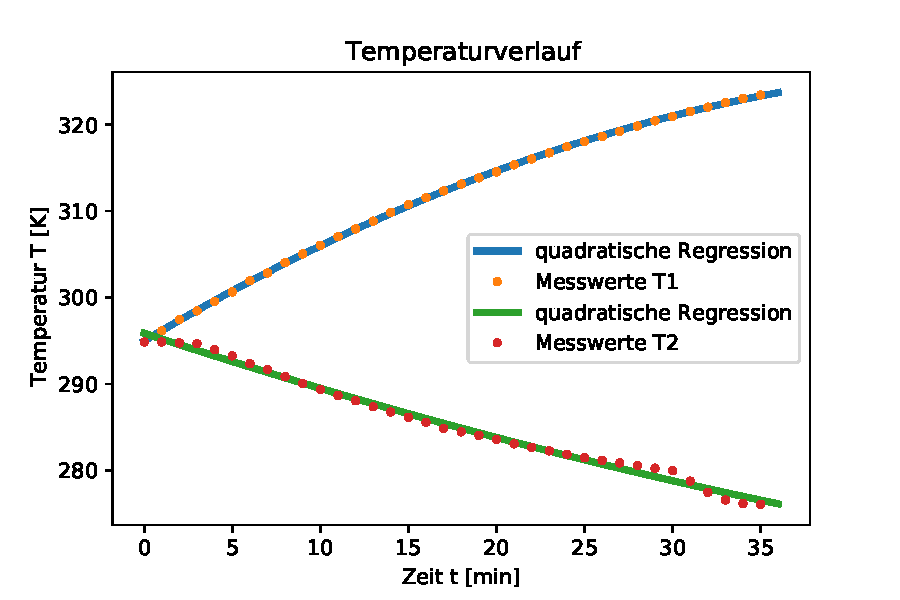
\includegraphics{Temperaturverlauf.pdf}
  \caption{Temperaturverlauf}
  \label{fig:Temperaturverlauf}
\end{figure}

\begin{center}
$T(t)=At^2 + Bt +C $
\end{center}

mit folgenden Faktoren für $T_1$: 

\begin{center}
$A_1=-0,012\pm0$ , $B_1=1,217\pm0,005$ , $C_1=294,97\pm0,041$
\end{center}



und folgenden Faktoren für $T_2$:
\begin{center}
$A_2=0,003\pm0,001$ , $B_2=-0,673\pm0,035$ , $C_2=295,870\pm0,263$
\end{center}
Alle Faktoren wurden duch die Numpy Polyfit Funktion berechnet. 

\subsection{Aufgabe 5c Berechnung der Differentialkoeffizeinten:}
\noindent Im nächsten Schritt werden die Differentialkoeffizeinten der Ausgleichskurven
berechnet, dazu werden die an die Temperaturverläufe von $T_1$ und $T_2$ angenäherten 
quadratischen Funktionen differenziert.
\begin{center}
  $T_1=-0,012\pm0t^2+1,217t\pm0,005+294,97\pm0,041$\\
  $\Rightarrow\dot{T_1}=-0,024\pm0t+(1,217\pm0,005)$ \\
  $T_2=0,003\pm0,001t^2-0,673\pm0,035t+295,870\pm0,263$\\
  $\Rightarrow\dot{T_2}=0,006\pm0,002t-1,346\pm0,005$

\end{center}

\noindent In der nachfolgenden Tabelle wurden die Differentiale der Ausgleichskurven $\dot{T_1}$ und
$\dot{T_2}$ an vier willkürlich ausgesuchten Stellen $t$ ausgewertet und zusammen mit 
dem gewählten Zeitpunkt und der entsprechenden Kompressorleistung aufgeführt.

\begin{table}
  \centering
  \label{Differentialquotienten}
  \caption{Delta T}
  \sisetup{table-format=1.2}
  \begin{tabular}{S[table-format=4.2] S S S S S [table-format=4.2]}
    \toprule
    {$t [min]$} & {$\dot{T_1}$} & {$\dot{T_2}$} & {$\bar{N}$} \\
    \midrule
    7   & {$1,049\pm0,005$} & {$-0.750\pm0,04$} &  120 \\
    14  & {$0,881\pm0,005$} & {$-0,498\pm0,04$} &  120 \\
    21  & {$0,713\pm0,005$} & {$-0,246\pm0,05$} &  120 \\
    28  & {$0,545\pm0,005$} & {$ 0,006\pm0,05$} &  122 \\
    \bottomrule
    
  \end{tabular}
\end{table}

\subsection{Aufgabe 5d Berechnung der Güteziffer}
Die reale Güteziffer $v_{real}$ berechnet sich über folgenden Ausdruck:
\begin{center}
  $v_{real}=\frac{\increment Q_1}{\increment t N}$
\end{center}

Mit der pro Zeiteinheit gewonnenen Wärmemenge:
\begin{center}
  $\frac{\increment Q_1}{\increment t}=(m_1 c_w + m_k c_k) \dot{T_1}$
\end{center}

Wärmekapazität Wasser für $m_1=4kg$ und $c_w=16,736\frac{J}{kg*K}$:
\begin{center}
  $m_1 c_w=66,944\frac{J}{K}$ 
\end{center}

Wärmekapazität Kupferschlange und Behälter:
\begin{center}
  $m_k c_k=750\frac{J}{K}$
\end{center}

Die theoretische Güteziffer $v_{theorie}$ berechnet sich durch:
\begin{center}
  $v_{theorie}=\frac{T_1}{T_1-T_2}$
\end{center}
\begin{table}
  \centering
  \label{Differentialquotienten}
  \caption{Güteziffern}
  \sisetup{table-format=1.2}
  \begin{tabular}{S[table-format=3.2] S S S [table-format=3.2]}
    \toprule
    {$t [min]$} & {$v_{real}$} & {$v_{thorie}$} & {$\increment v$} \\
    \midrule
    7  & {$7,141\pm0,034$} & {$27,040\pm0,340$} & {$19,90\pm0,34$}\\
    14 & {$5,998\pm0,034$} & {$13,410\pm0,080$} & {$ 7,42\pm0,09$}\\
    21 & {$4,854\pm0,034$} & {$9,760\pm0,040$}  & {$ 4,91\pm0,05$}\\
    28 & {$4,774\pm0,033$} & {$8,139\pm0,028$}  & {$ 3,36\pm0,04$}\\
    \bottomrule
    
  \end{tabular}
\end{table}
$\increment v $ bezeichnet die Abweichung zwischen der realen Güteziffer $v_{real}$ und der theoretische 
Güteziffer $v_{theorie}$
\newpage

\subsection{Aufgabe 5e Der Massendurchsatz}
Der Massendurchsatz lässt sich nach folgender Vorschrift berechnen:

\begin{center}
  $\frac{\increment m}{\increment t}=(m_2 c_w + m_k c_k)\frac{\dot{T_2}}{L}$
\end{center}
\subsubsection{Berchnung von L}
Zur Berechnung der Verdampfungswärme $L$ wird der ln$(p_2)$ gegen $\frac{1}{T_2}$ aufgetragen und eine 
Ausgleichsgerade bestimmt aus deren Steigung man mit $L=-\frac{m}{R}$ die gesuchte Größe berechnen kann.

\begin{figure}
  \centering
  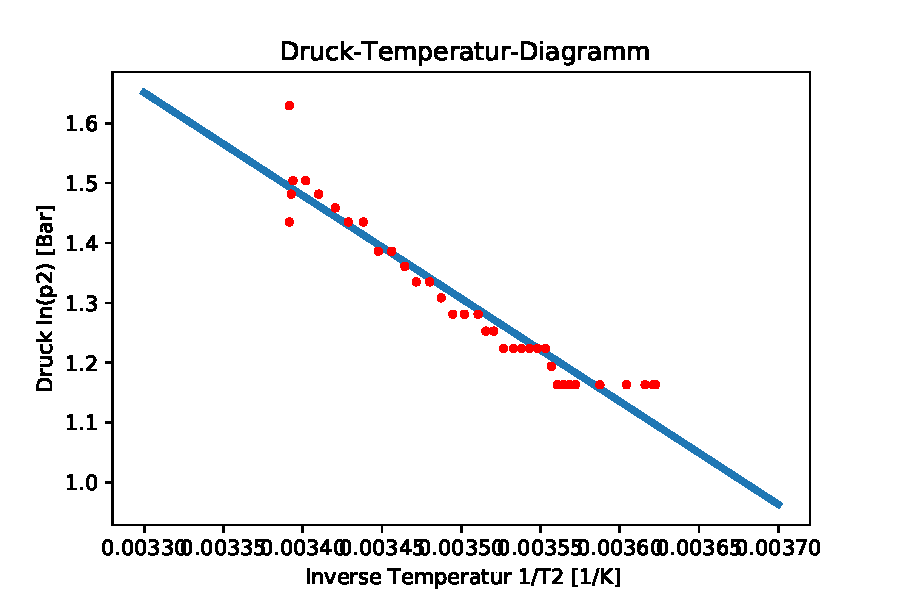
\includegraphics{Drucktemperaturdiagram.pdf}
  \caption{Dampfdruck-Kurve}
  \label{fig:DampfdruckKurve}
\end{figure}

\noindent Die durch die Numpy Polyfit Funktion bestimmte Steigung $m=-1719.830\pm88.369$ lefert mit der allgemeinen Gaskonstante
$R=8,314\frac{kg*m^2}{s^2*mol*K}$ den Wert für $L=207\pm11\frac{kg^2*m^2}{s^4*mol}$.
Die Fitfunktion lautet:$f(T)=\frac{-1719.830\pm88.369}{T}+7.327\pm0.310$

\subsubsection{Berechnung des Massendurchsatzes}
Für den Massendurchsatz ergeben sich also folgende Werte:
\begin{center}
  $\frac{\increment m}{\increment t}=(m_2 c_w + m_k c_k)\frac{\dot{T_2}}{L}$
\end{center}
mit:
\begin{center}
  $m_2=4kg$\\
  $c_w=16,736\frac{J}{kg*K}$\\
  $m_2 c_w=66,944\frac{J}{K}$\\
  $m_k c_k=750\frac{J}{K}$
\end{center}

\begin{center}
  $(\frac{\increment m}{\increment t})_1=-2.49\pm0.20\frac{kg}{s}$\\
  $(\frac{\increment m}{\increment t})_2=-2.33\pm0.21\frac{kg}{s}$\\
  $(\frac{\increment m}{\increment t})_3=-2.16\pm0.24\frac{kg}{s}$\\
  $(\frac{\increment m}{\increment t})_4=-2.16\pm0.24\frac{kg}{s}$\\
\end{center}

\subsection{Aufgabe 5e Berechnung der Mechanischen Kompressorleistung}

Die Mechanische Kompressorleistung berechnet sich wie folgt:

\begin{center}
  $N_{mech}=\frac{1}{\kappa-1}(p_2\sqrt[\kappa]{\frac{p_1}{p_2}}-p_1)\frac{1}{\rho}\frac{\increment m}{\increment t}$\\
\end{center}
mit:
\begin{center}
  $\rho=\frac{\rho_0 T_0 p_1}{T_2 p_0}$
\end{center}
  mit folgenden Werten für $Cl_2F_2C:$\\
\begin{center}
$\rho_0=5,51\frac{g}{L}$\\
$\kappa=1,14$\\
$T_0=273,15\pm0,1K$\\
$p_0=5,1Bar$
\end{center}
ergeben sich diese Werte:
\begin{table}
  \centering
  \label{Differentialquotienten}
  \caption{Kompressorleistung}
  \sisetup{table-format=1.2}
  \begin{tabular}{S[table-format=3.2] S S S [table-format=3.2]}
    \toprule
    {$t [min]$} & {$\rho$} & {$N [W]$} \\
    \midrule
    7  & 7,589 & {$1.21\pm0.10$}\\
    14 & 9,262 & {$1.67\pm0.15$}\\
    21 & 10,426 & {$1.84\pm0.21$}\\
    28 & 12,097 & {$2.13\pm0.24$}\\
    \bottomrule
    
  \end{tabular}
\end{table}

\newpage
\subsection{Aufgabe 5g Gründe für die schlechte Güteziffer}
Gründe für die schlechte Güteziffer sind in den nicht idealen Bedingungen
eines realen Versuchsaufbaus zu finden. Da der Versuch jedoch nicht 
real durchgeführt wurde sind diese nicht offensichtlich und es können 
nur Mutmaßungen angestellt werden. Zu diesen Mutmaßungen gehören: eine nicht perfekte Isolierung der
Reservoire und deren Verbindungen, und eventuell unpräzise oder schlecht ablesbare 
Messinstrumente.